
\subsection*{All Orthonormal Bases for $\mathbb{R}^2$}

%%%Insert this to get the typewriter font so it looks like a real movie script
{\ttfamily
\fontdimen2\font=0.4em
\fontdimen3\font=0.2em
\fontdimen4\font=0.1em
\fontdimen7\font=0.1em
\hyphenchar\font=`\-


\hypertarget{scripts_orthonormal_bases_sin_cos}{We wish to find all orthonormal bases for} the space $\mathbb{R}^2$, and they are $\{ e_1^{\theta}, e_2^{\theta} \}$ up to reordering where
\[
\begin{array}{cc}
e_1^{\theta} = \begin{pmatrix} \cos \theta \\ \sin \theta \end{pmatrix}, & e_2^{\theta} = \begin{pmatrix} -\sin \theta \\ \cos \theta \end{pmatrix},
\end{array}
\]
for some $\theta \in [0, 2\pi)$. Now first we need to show that for a fixed $\theta$ that the pair is orthogonal:
\[
e_1^{\theta} \dotprod e_2^{\theta} = -\sin \theta \cos \theta + \cos \theta \sin \theta = 0.
\]
Also we have
\[
\norm{e_1^{\theta}}^2 = \norm{e_2^{\theta}}^2 = \sin^2 \theta + \cos^2 \theta = 1,
\]
and hence $\{ e_1^{\theta}, e_2^{\theta} \}$ is an orthonormal basis. To show that every orthonormal basis of $\mathbb{R}^2$ is $\{ e_1^{\theta}, e_2^{\theta} \}$ for some $\theta$, consider an orthonormal basis $\{ b_1, b_2 \}$ and note that $b_1$ forms an angle $\phi$ with the vector $e_1$ (which is $e_1^0$). Thus $b_1 = e_1^{\phi}$ and if $b_2 = e_2^{\phi}$, we are done, otherwise $b_2 = -e_2^{\phi}$ and it is the reflected version. However we can do the same thing except starting with $b_2$ and get $b_2 = e_1^{\psi}$ and $b_1 = e_2^{\psi}$ since we have just interchanged two basis vectors which corresponds to a reflection which picks up a minus sign as in the determinant.

%\begin{figure}[ht!]
%\label{figure:sin_cos_onb}
\begin{center}
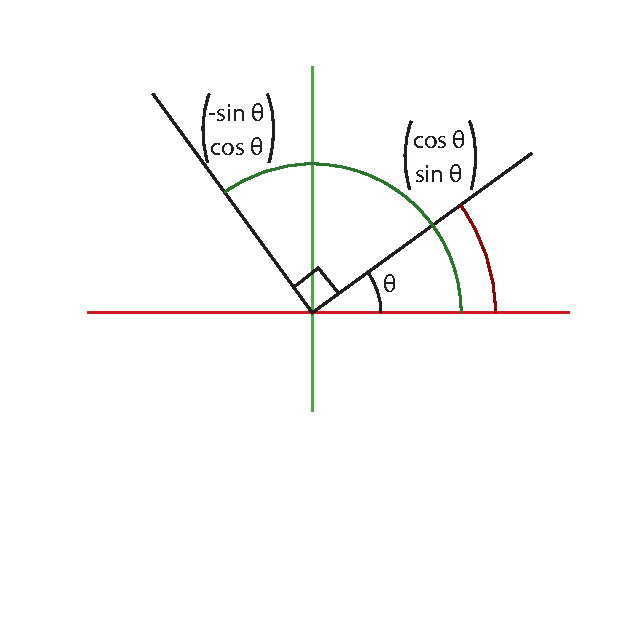
\includegraphics[scale=1.1]{\orthonormPath/sin_cos_onb.pdf}
\end{center}
%\caption{Plot of the vectors $e_1^{\theta}$ and $e_2^{\theta}$ in $\mathbb{R}^2$.}
%\end{figure}

} % Closing bracket for font

%\newpage
